\documentclass{beamer}

\usepackage[utf8]{inputenc}
\usepackage[brazil]{babel}

\usepackage{verbatim}
\usepackage{multirow}

\usepackage{graphicx}
%\usepackage[table]{xcolor}
\usepackage{listings}
\usepackage{color}

\definecolor{mygreen}{rgb}{0,0.6,0}
\definecolor{mygray}{rgb}{0.5,0.5,0.5}
\definecolor{mymauve}{rgb}{0.58,0,0.82}
\definecolor{mybckg}{rgb}{0.95,0.95,0.95}
\lstset{
  backgroundcolor=\color{mybckg},  % choose the background color; you must add \usepackage{color} or \usepackage{xcolor}
  basicstyle=\footnotesize,       % the size of the fonts that are used for the code
  breakatwhitespace=false,         % sets if automatic breaks should only happen at whitespace
  breaklines=true,                 % sets automatic line breaking
  %captionpos=b,                    % sets the caption-position to bottom
  %commentstyle=\color{mygreen},    % comment style
  deletekeywords={...},            % if you want to delete keywords from the given language
  escapeinside={\%*}{*)},          % if you want to add LaTeX within your code
  extendedchars=true,              % lets you use non-ASCII characters; for 8-bits encodings only, does not work with UTF-8
  frame=single,                    % adds a frame around the code
  keepspaces=true,                 % keeps spaces in text, useful for keeping indentation of code (possibly needs columns=flexible)
  columns=flexible,
  %keywordstyle=\color{blue},       % keyword style
  %language=bash,                   % the language of the code
  morekeywords={*,...,Hello,LS,Update},            % if you want to add more keywords to the set
  %numbers=left,                    % where to put the line-numbers; possible values are (none, left, right)
  %numbersep=5pt,                   % how far the line-numbers are from the code
  %numberstyle=\tiny\color{mygray}, % the style that is used for the line-numbers
  rulecolor=\color{black},         % if not set, the frame-color may be changed on line-breaks within not-black text (e.g. comments (green here))
  %showspaces=false,                % show spaces everywhere adding particular underscores; it overrides 'showstringspaces'
  %showstringspaces=false,          % underline spaces within strings only
  %showtabs=false,                  % show tabs within strings adding particular underscores
  %stepnumber=2,                    % the step between two line-numbers. If it's 1, each line will be numbered
  %stringstyle=\color{mymauve},     % string literal style
  tabsize=2,                       % sets default tabsize to 2 spaces
  %title=\lstname                   % show the filename of files included with \lstinputlisting; also try caption instead of title
  literate=
  {á}{{\'a}}1 {é}{{\'e}}1 {í}{{\'i}}1 {ó}{{\'o}}1 {ú}{{\'u}}1
  {Á}{{\'A}}1 {É}{{\'E}}1 {Í}{{\'I}}1 {Ó}{{\'O}}1 {Ú}{{\'U}}1
  {à}{{\`a}}1 {è}{{\'e}}1 {ì}{{\`i}}1 {ò}{{\`o}}1 {ù}{{\`u}}1
  {À}{{\`A}}1 {È}{{\'E}}1 {Ì}{{\`I}}1 {Ò}{{\`O}}1 {Ù}{{\`U}}1
  {ä}{{\"a}}1 {ë}{{\"e}}1 {ï}{{\"i}}1 {ö}{{\"o}}1 {ü}{{\"u}}1
  {Ä}{{\"A}}1 {Ë}{{\"E}}1 {Ï}{{\"I}}1 {Ö}{{\"O}}1 {Ü}{{\"U}}1
  {â}{{\^a}}1 {ê}{{\^e}}1 {î}{{\^i}}1 {ô}{{\^o}}1 {û}{{\^u}}1
  {Â}{{\^A}}1 {Ê}{{\^E}}1 {Î}{{\^I}}1 {Ô}{{\^O}}1 {Û}{{\^U}}1
  {œ}{{\oe}}1 {Œ}{{\OE}}1 {æ}{{\ae}}1 {Æ}{{\AE}}1 {ß}{{\ss}}1
  {ç}{{\c c}}1 {Ç}{{\c C}}1 {ø}{{\o}}1 {å}{{\r a}}1 {Å}{{\r A}}1
  {€}{{\EUR}}1 {£}{{\pounds}}1,
  %basicstyle=\ttfamily
}

\useoutertheme{infolines} % add a footline 
\usetheme{Frankfurt}
%\setbeamertemplate{items}[square] % changes the markers, ball: 3-dimensional balls, circle: 2-dimensional (flat) circles, rectangle: rectangles, default: triangles 
%\setbeamertemplate{section in toc}[circle]
\setbeamertemplate{section in toc}[ball unnumbered]
\setbeamertemplate{enumerate item}[square]
\setbeamertemplate{itemize item}[triangle]
\setbeamertemplate{itemize subitem}[circle]
\setbeamertemplate{blocks}[rounded][shadow=true] % add rounded corners and a shadow to the box that surrounds the theorem
\setbeamertemplate{navigation symbols}{} % disable the drawing of navigation icons

\newlength{\wideitemsep}
\setlength{\wideitemsep}{\itemsep}
\addtolength{\wideitemsep}{10pt}
\let\olditem\item
\renewcommand{\item}{\setlength{\itemsep}{\wideitemsep}\olditem}

\title[Aplicações escaláveis com MEAN \textit{Stack}]{Aplicações escaláveis com MEAN \textit{Stack}}
\author[Filipe Leuch Bonfim, Michael Liang]{Filipe Leuch Bonfim \\ Michael Liang}
\institute[UFPR]{
  Departamento de Informática\\
  Universidade Federal do Paraná\\
  Bacharelado em Ciência da Computação\\
  Trabalho de Graduação\\
  Orientador: Prof. Bruno Muller Junior.
}

\usepackage{remreset}
\makeatletter
\@removefromreset{subsection}{section}
\makeatother


\begin{document}
%\maketitle

\begin{comment}
\frame{\titlepage}

\frame{
\frametitle{Sumário}
\tableofcontents
}
\end{comment}

\begin{frame}
  \titlepage
\end{frame}

\section*{Sumário}
\begin{frame}
\tableofcontents
\end{frame}

\setcounter{subsection}{1}

%\section{Introduçao}

\section{Conceitos}

\begin{frame}{Aplicações web escaláveis}
    \begin{description}
        \item[Escalabilidade] \hfill \\
        \item[Aplicações web] \hfill \\
        \item[Escalabilidade em aplicações web] \hfill \\
    \end{description}
\end{frame}

\begin{frame}{Escalabilidade}
    Escalabilidade é a habilidade de uma aplicação manter o desempenho
quando a carga de trabalho aumenta.
\end{frame}

%\begin{frame}{Escalabilidade - Internet}
%    \begin{figure}[htb]
%    \centering
%    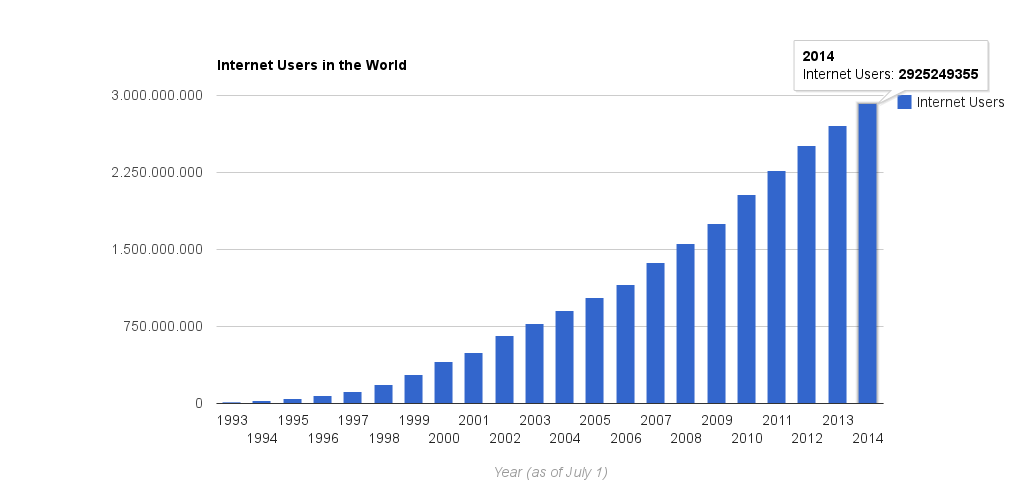
\includegraphics[scale=0.32]{../images/internet_usage.png}
%    \caption{ Quantidade de usuários da internet entre 1993 e 2014 }
%    \label{fig: graf_iu}
%    \end{figure}
%\end{frame}

\begin{frame}{Aplicações web}
A aplicação web refere-se a sistemas de informática que são executados através de navegadores com internet, geralmente aplicações que utilizam-se de tecnologias web como HTML, Javascript e CSS.
\end{frame}

%\begin{frame}{Escalabilidade em aplicações web}
%    \begin{itemize}
%        \item Escalabilidade vertical
%        
%        \hfill É quando existe uma melhoria do hardware de um único servidor. 
%        \item Escalabilidade horizontal 
%        
%        \hfill Significa adicionar mais servidores, permitindo a criação de um \textit{cluster}.
%    \end{itemize}
%\end{frame}

\begin{frame}{Escalabilidade vertical e horizontal}
  \begin{figure}[htb]
    \centering
    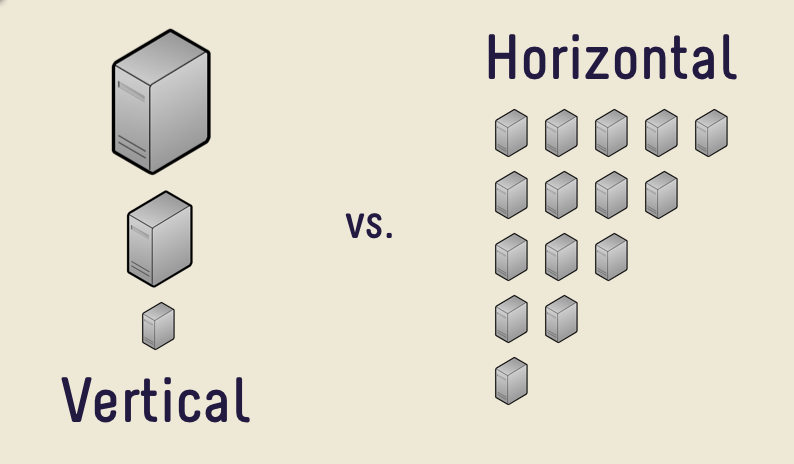
\includegraphics[scale=0.30]{../images/scal_vh.png}
    \caption{ Escalabilidade vertical e horizontal}
    \label{fig: scal_vh}
    \end{figure}
\end{frame}

\begin{frame}{Programação orientada a eventos}
    \begin{itemize}
        \item É um paradigma de programação  
        
         \item É um laço que recebe repetidamente informação para processar e disparam uma função de resposta de acordo com o evento recebido.
         
        \item Um evento é qualquer ação do usuário que interaja com o sistema.
        \end{itemize}
\end{frame}

\begin{frame}{Programação orientada a eventos - Event Loop}
    \begin{figure}[htb]
    \centering
    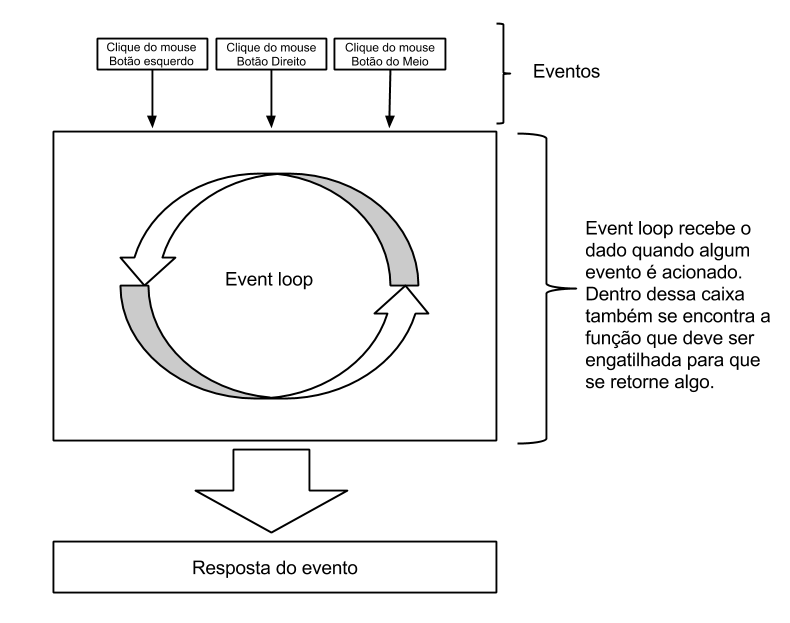
\includegraphics[scale=0.30]{../images/event_loop_diagram.png}
    \caption{Event Loop}
    \label{fig: graf_eld}
    \end{figure}
\end{frame}

\begin{frame}{Javascript}
    \begin{description}
        %\item[Imperativa e estruturada] \hfill \\
        \item[Tipagem dinâmica] \hfill \\
        \item[Baseada em protótipos] \hfill \\
        \item[Linguagem orientada a eventos] \hfill \\
    \end{description}
\end{frame}

\begin{frame}{NoSQL - Not Only SQL}
    \begin{itemize}
        \item Costuma ser projetado para ser executado em um \textit{cluster};
        \item Costuma ser Open-Source; 
        \item Não possui esquema fixo (SCHEMA-LESS), permitindo gravar qualquer dado em qualquer estrutura.
        \item Categorias: Chave/Valor, Orientado a colunas, Orientado a documentos, Baseado em grafos
    \end{itemize}
\end{frame}

\section{Tecnologias}

\begin{frame}{MEAN \textit{Stack}}
\begin{itemize}
        \item MongoDB
        \item Express.js
        \item AngularJS
        \item Node.js
    \end{itemize}
\end{frame}

\begin{frame}{MongoDB}
    \begin{itemize}
        \item NoSQL 
        \item Orientado a documentos
        \item O formado dos documentos é JSON/BSON
     \end{itemize}
\end{frame}

%\begin{frame}{MongoDB - Termos/Conceitos}
%    \begin{table}[ht]
%    \begin{tabular}{|p{5cm}|p{5cm}|}
%    \hline
    %\rowcolor[HTML]{CFCFCF} 
%    Termos/Conceitos SQL & Termos/Conceitos MongoDB \\ \hline
%    base de dados        & base de dados          \\ \hline
%    tabela               & coleção                \\ \hline
%    linha                & documento (BSON)       \\ \hline
%    coluna               & campo                  \\ \hline
%    índice               & índice                 \\ \hline
%    joins                & documentos incorporados (\textit{embedded})                                            \\ \hline
%    chave primária       & chave primária         \\ \hline
%                         &                        \\
%                         &                        \\
%    \multirow{-3}{5cm}{Especificar uma coluna ou um conjunto   de colunas como chave primária} & \multirow{-3}{5cm}{No MongoDB, a chave primária é  automaticamente atribuída ao campo \_id} \\ \hline
%    \end{tabular}
%    \caption{Comparação entre as terminologias do SQL e do MongoDB.}
%    \label{fig:tab_mg_sql}
%    \end{table}
%\end{frame}

\begin{frame}{MongoDB - Escalabilidade através do Sharding}
    \begin{figure}[htb]
    \centering
    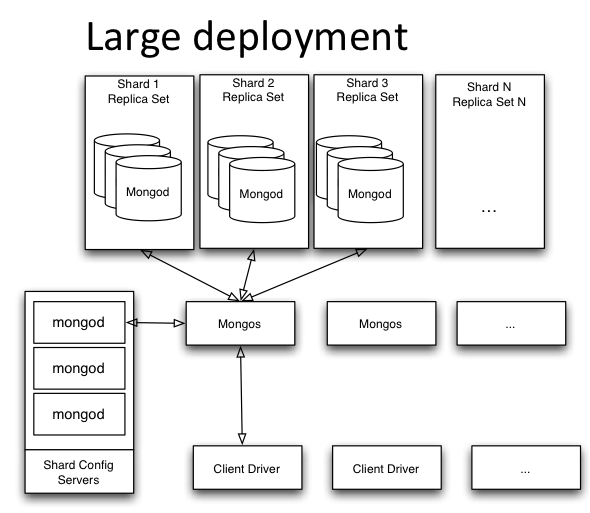
\includegraphics[scale=0.35]{../images/1sharding_topology.png}
    \caption{Topologia do Sharding}
    \label{fig: shard_top}
    \end{figure}
\end{frame}

\begin{frame}{MongoDB - Armazenamento}
    \begin{itemize}
        \item Utiliza arquivos mapeados
em memória.
        \item Consistência eventual
    \end{itemize}
\end{frame}

\begin{frame}{Express.js}

    \begin{itemize}
        \item O Express é um \textit{framework} que visa facilitar o desenvolvimento de aplicações Web com o Node.js.
        \item O Express.js permite criar servidores web e receber requisições HTTP de maneira simples. 
        \item  Ele também permite a criação de um conjunto de diretórios com uma estrutura padrão, além de organizar as rotas dos arquivos para as \textit{views} da aplicação.
        \item  Geralmente os projetos que utilizam-se do Express também aderem há algum \textit{framework} de \textit{templates} como Jade ou EJS.
    \end{itemize}
\end{frame}

 
\begin{frame}{AngularJS}
    \begin{itemize}
        \item Framework Javascript \textit{client-side}
        \item MVC
    \end{itemize}
\end{frame}

\begin{frame}{AngularJS - Comparando com outros frameworks}
    \begin{figure}[htb]
    \centering
    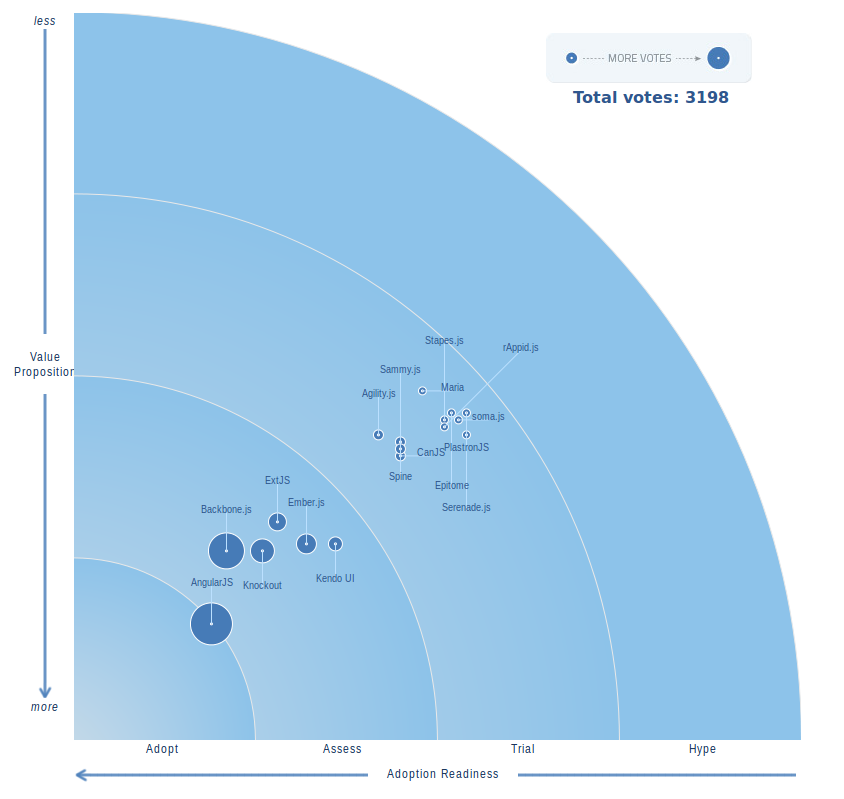
\includegraphics[scale=0.22]{../images/angularjs_framework_comparison.png}
    \caption{Gráfico comparando frameworks Javascript.}
    \label{fig: ang_fw_comp}
    \end{figure}
\end{frame}

\begin{frame}{AngularJS - Características}
    \begin{description}
        \item[SPA - Single Page Application] \hfill \\
            Cada parte de página é carregada de forma independente.
        \item[Injeção de dependências] \hfill \\
            Fornecer recursos extras necessários na aplicação de forma transparente ao usuário. Ex: ng-Resources, ng-Routes, etc.
        \item[Two-Way Data Biding] \hfill \\
            Sincroniza os dados na \textit{view} e no \textit{model}.

    \end{description}
\end{frame}

\begin{frame}{AngularJS - Características}
    \begin{figure}[htb]
    \centering
    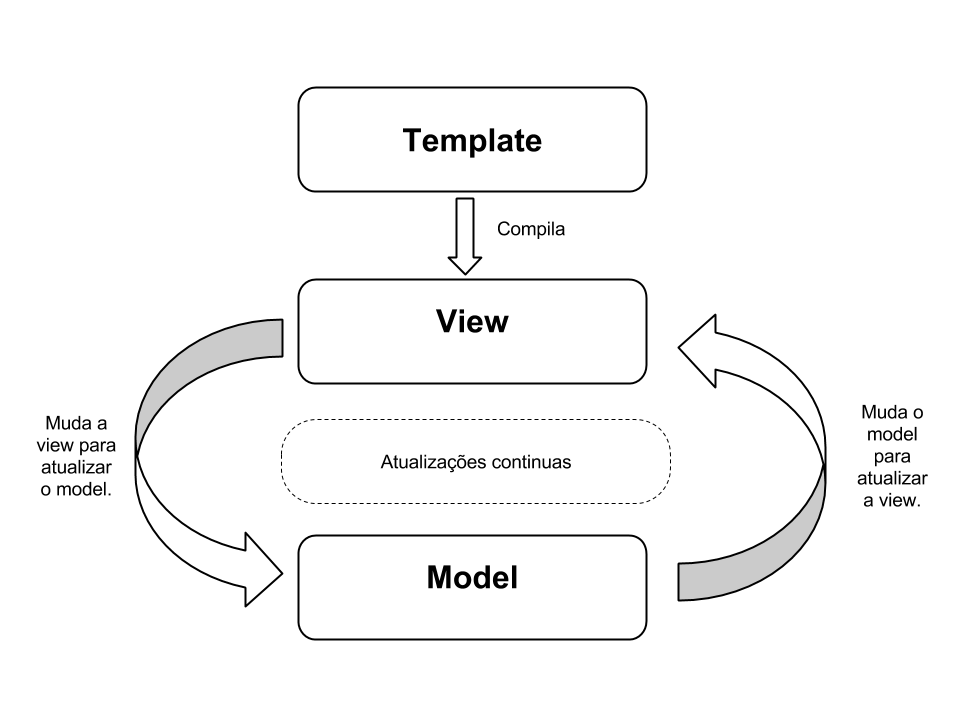
\includegraphics[scale=0.20]{../images/Two_way_databiding_diagram.png}
    \caption{Digrama do \textit{Two-way data biding}}
    \label{fig: twdb}
    \end{figure}
\end{frame}

\begin{frame}{Node.js}
    \begin{itemize}
        \item É uma plataforma de desenvolvimento web
        \item Linguagem Javascript
no lado do servidor.
        \item Desenvolvida em C e Javascript
    \end{itemize}
\end{frame}

\begin{frame}{Node.js - Arquitetura}
    \begin{figure}[htb]
    \centering
    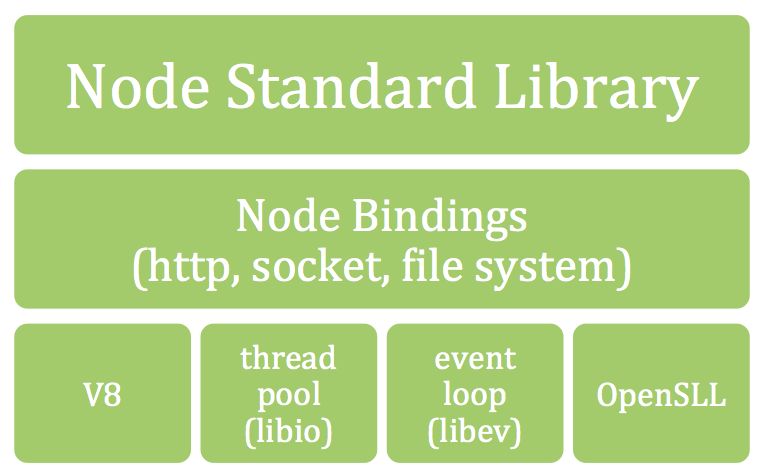
\includegraphics[scale=0.35]{../images/node_platform.png}
    \caption{Arquitetura do Node.js.}
    \label{fig: node_plat}
    \end{figure}
\end{frame}

\begin{frame}{Node.js - I/O não bloqueante e orientado a eventos}
    \begin{figure}[htb]
    \centering
    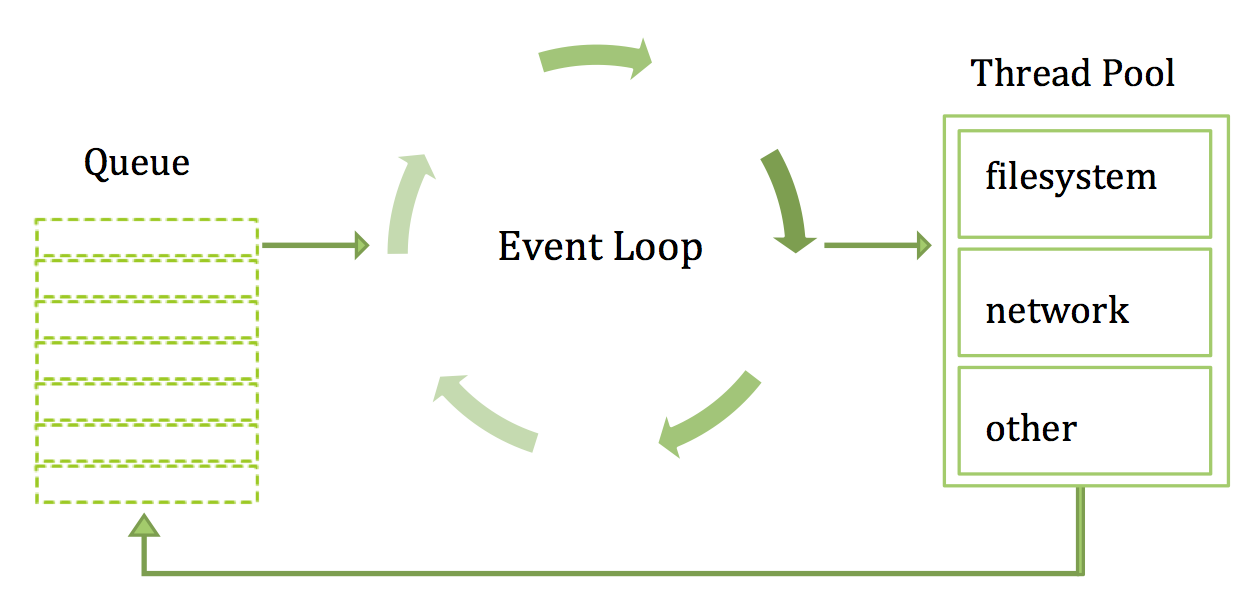
\includegraphics[scale=0.25]{../images/node_event_loop.png}
    \caption{Event Loop do Node.js.}
    \label{fig: node_el}
    \end{figure}
\end{frame}

%\begin{frame}{Socket.io}
%O Socket.io é uma API em Javascript que permite que a comunicação entre o servidor e o cliente ocorra sem dificuldades e em tempo real.
%\end{frame}

\section{Aplicações web com MEAN Stack} 

\begin{frame}{Aplicações web com MEAN \textit{Stack}}
    \begin{figure}[htb]
    \centering
    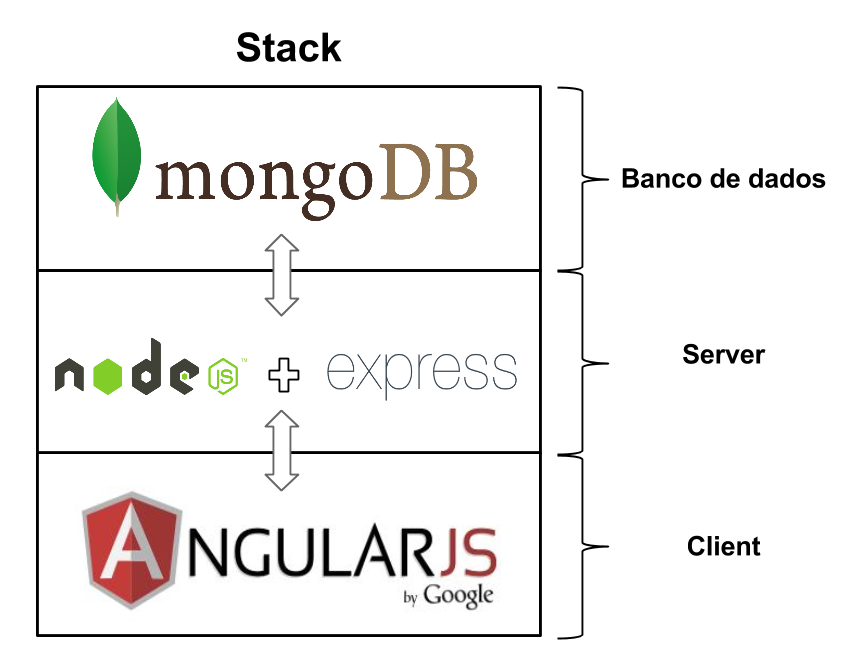
\includegraphics[scale=0.25]{../images/mean_stack_diagram.png}
    \caption{MEAN Stack visto como uma pilha}
    \label{fig: mean_diag}
    \end{figure}
\end{frame}

\begin{frame}{Comparativo em relação a arquitetura de aplicações LAMP}
    \begin{figure}[htb]
    \centering
    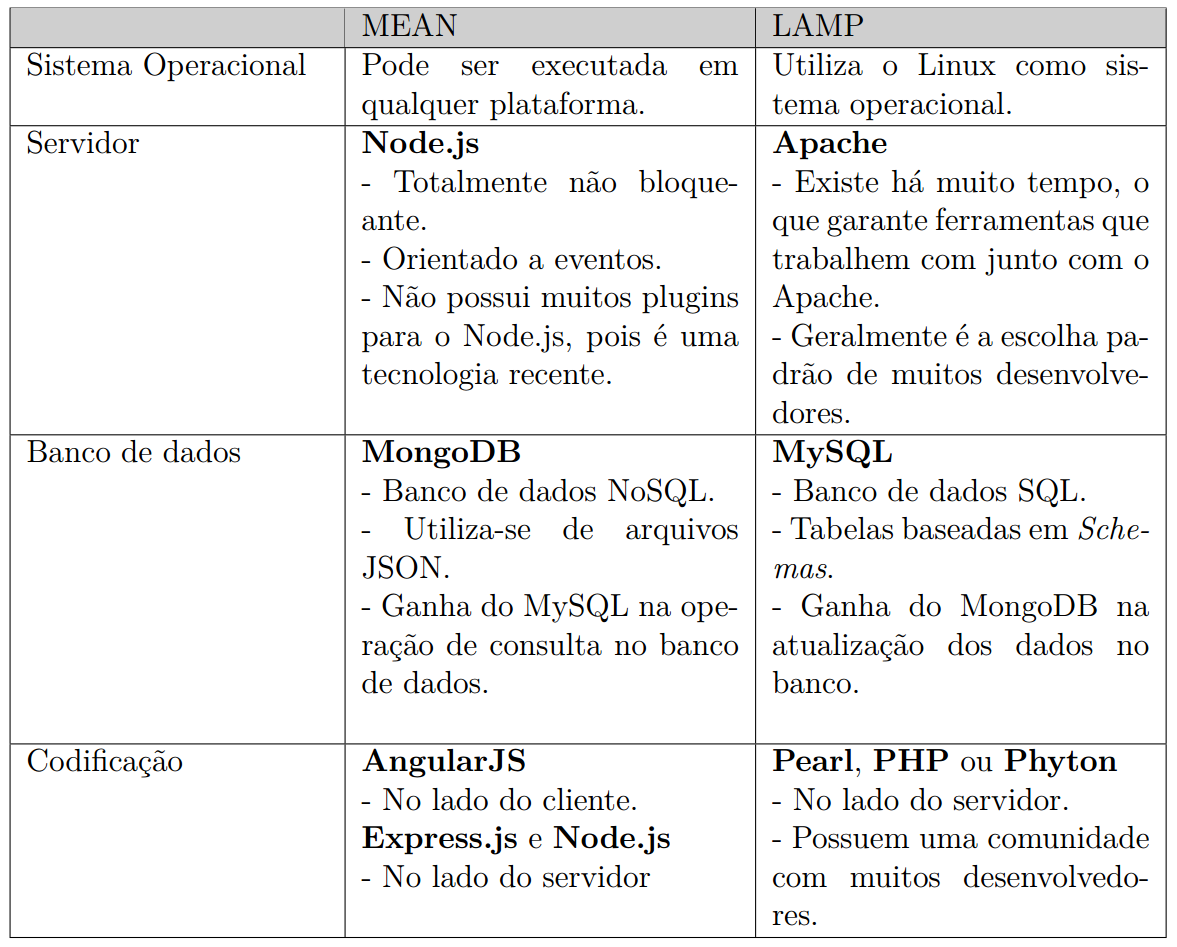
\includegraphics[scale=0.26]{../images/mean_lamp.png}
    \caption{MEAN Stack vs LAMP}
    \label{fig: mean_lamp}
    \end{figure}
\end{frame}

\begin{frame}{Math Race - Proposta da aplicação}
%\begin{itemize}
% \item Implementa o RSS \textit{fingerprinting}.
% \item O algoritmo utiliza o preceito da correlação espacial das localidades adjacentes.
% \item Obtém-se um conjunto de pontos que definem uma região de onde o aparelho possa estar.
% \item A posição final do aparelho 
%  e obtida através do centroide desse conjunto de pontos.
%\end{itemize}
    Aplicação \textit{Math Race} desenvolvida com MEAN \textit{Stack}, com intuito de demonstrar a organização e integração das ferramentas propostas.
\end{frame}

% \begin{frame}{Math Race - Utilização e funcionamento da aplicação}
%     \begin{figure}[htb]
%     \centering
%     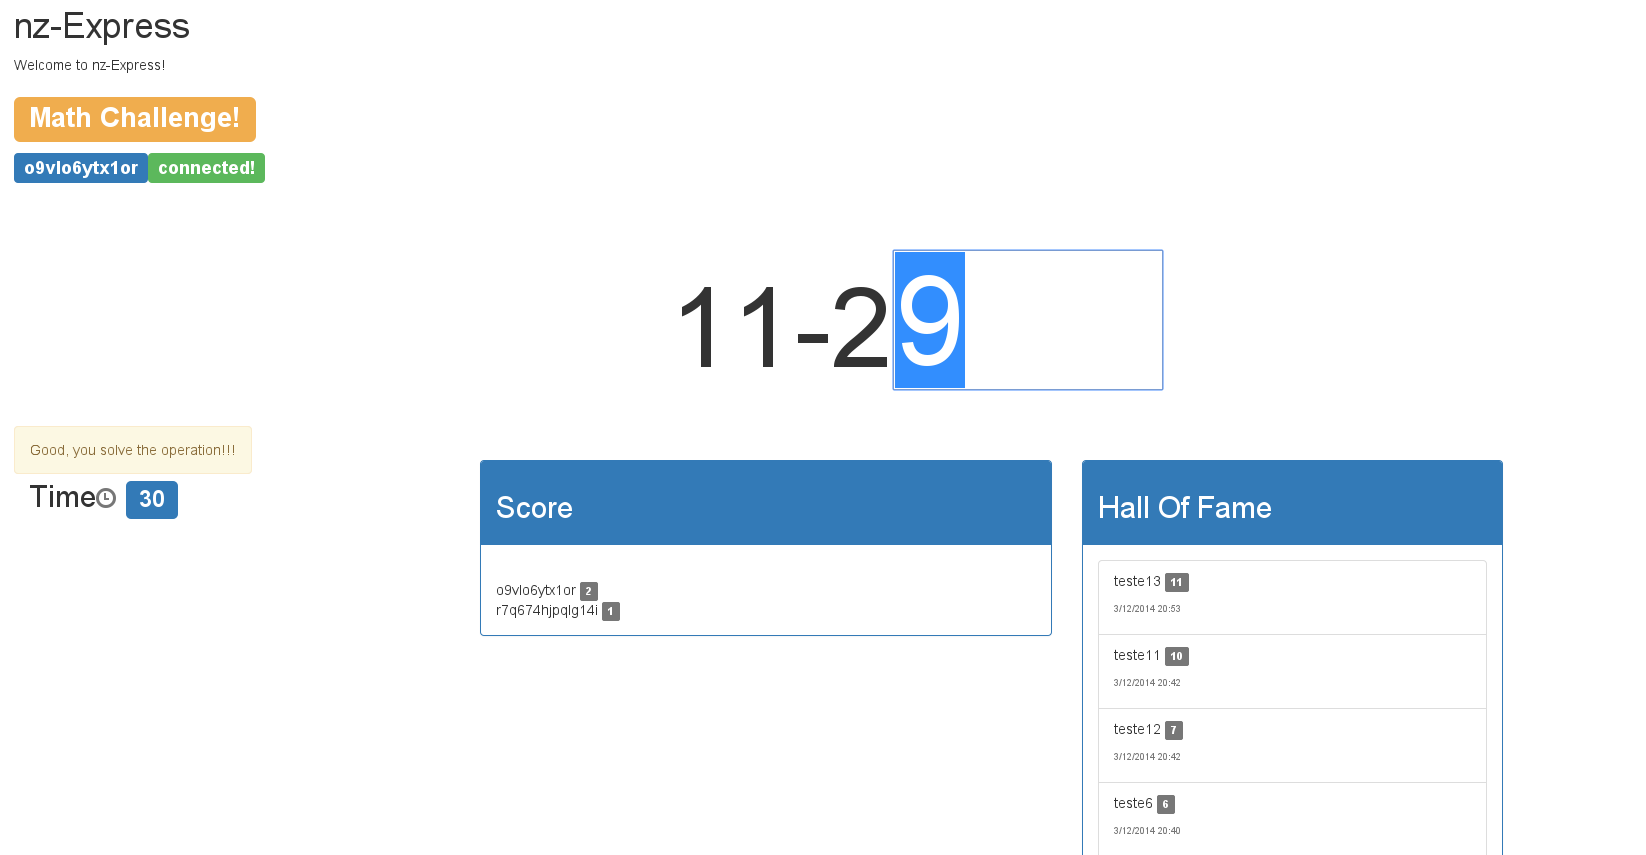
\includegraphics[scale=0.19]{../images/index_mean_math_race.png}
%     \caption{Imagem da interface da aplicação}
%     \label{fig: int_mr}
%     \end{figure}
% \end{frame}

\begin{frame}{Math Race - Desenvolvimento da aplicação}
\begin{figure}[htb]
    \centering
    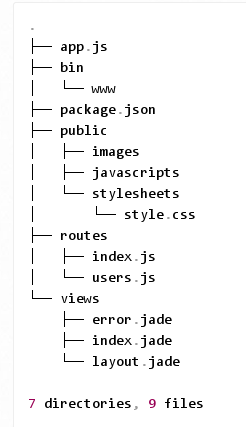
\includegraphics[scale=0.35]{../images/estrutura_exp_gen.png}
    \caption{Estrutura criada pelo express-generator}
    \label{fig: dir_mean_exp}
    \end{figure}
\end{frame}

\begin{frame}{Math Race - Integração das ferramentas do MEAN Stack}
    \begin{figure}[hbt]
    \centering
    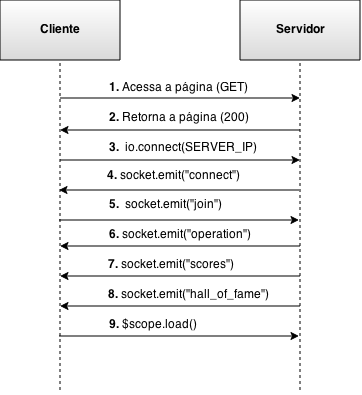
\includegraphics[scale=0.39]{../images/diagrama_de_seq_acesso.png}
    \caption{Diagrama de sequência do acesso da aplicação}
    \label{fig:appSchema}
    \end{figure}
\end{frame}

\begin{frame}{Math Race - Fluxo de execução}
    \begin{figure}[htb]
    \centering
    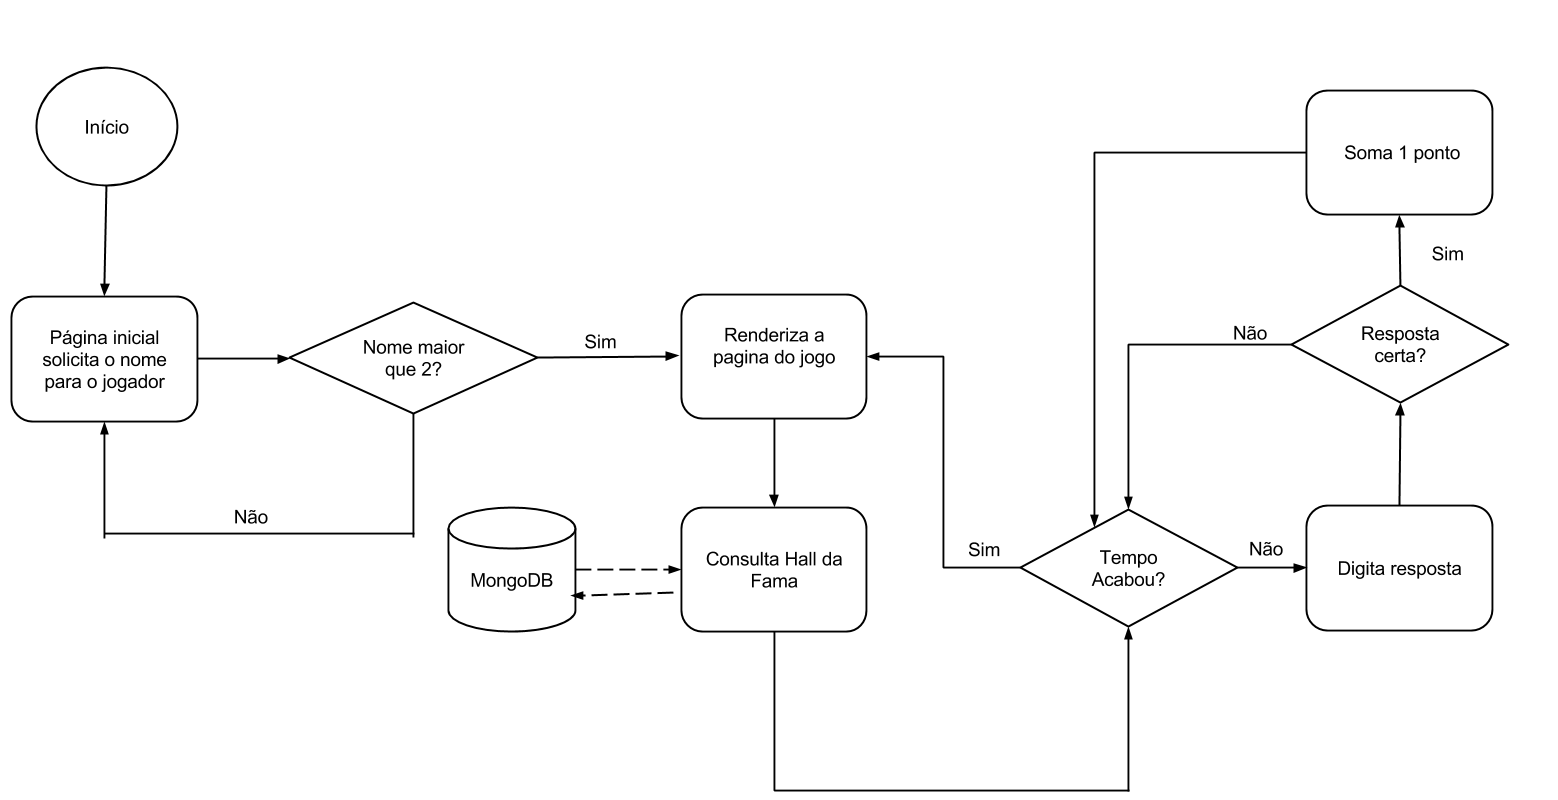
\includegraphics[scale=0.2]{../images/func_mr.png}
    \caption{Diagrama do funcionamento da aplicação}
    \label{fig: func_mr0}
    \end{figure}
\end{frame}
\begin{frame}{Math Race - Fluxo de execução}
    \begin{figure}[htb]
    \centering
    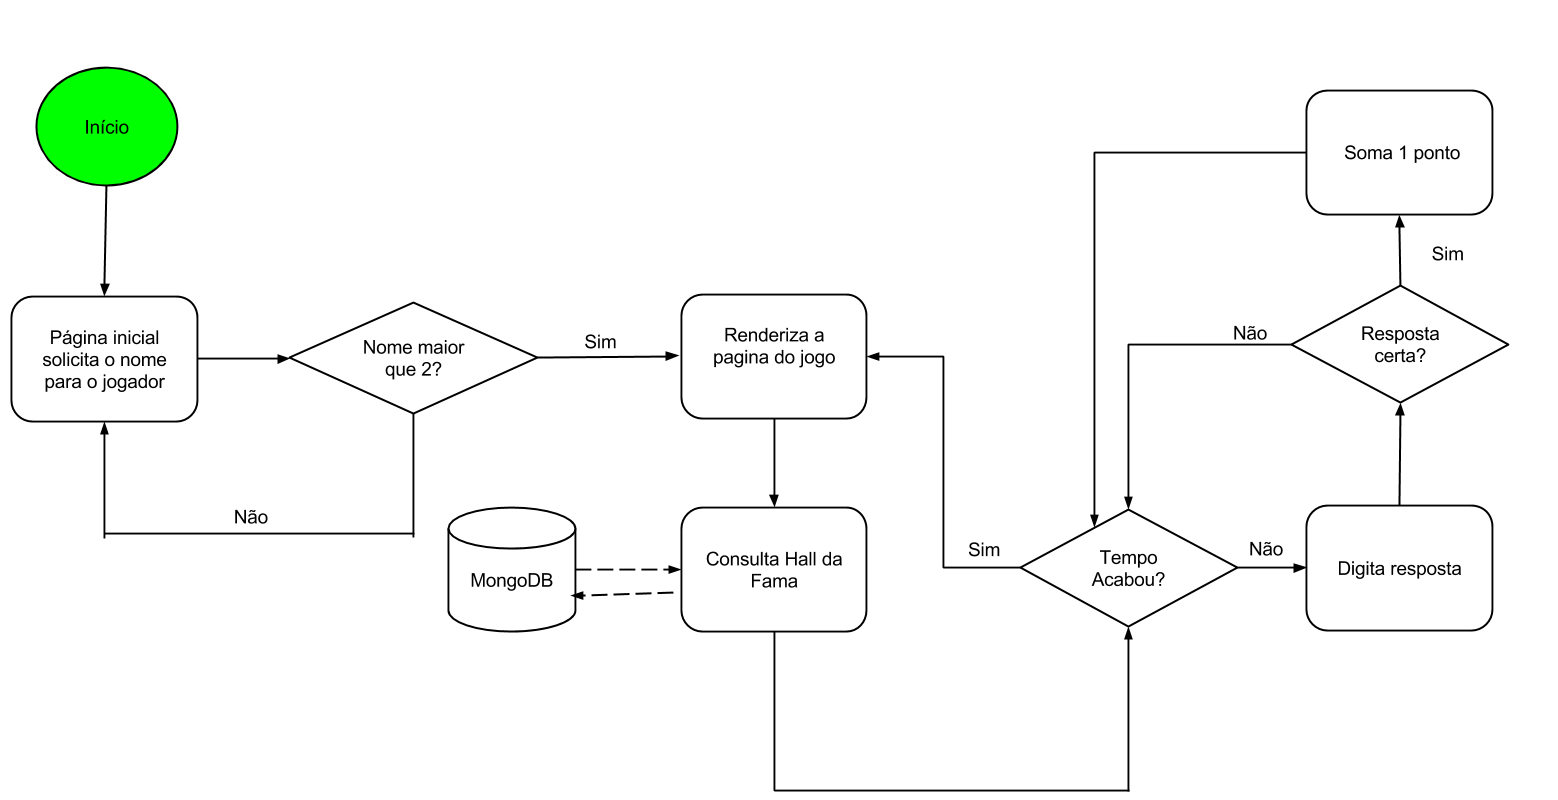
\includegraphics[scale=0.2]{../images/func_mr_s1.png}
    \caption{Diagrama do funcionamento da aplicação}
    \label{fig: func_mr1}
    \end{figure}
\end{frame}
\begin{frame}{Math Race - Fluxo de execução}
    \begin{figure}[htb]
    \centering
    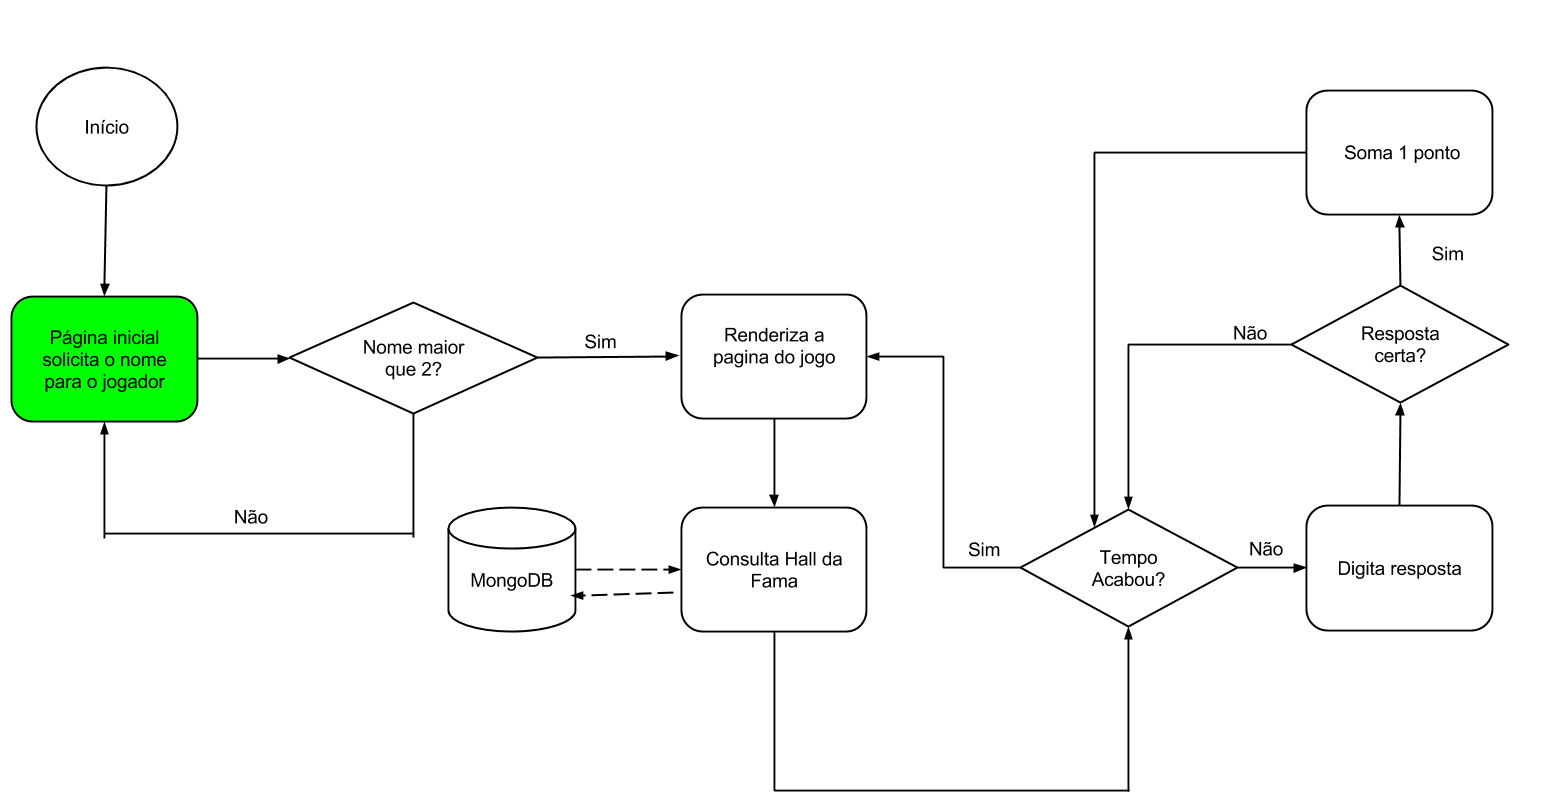
\includegraphics[scale=0.2]{../images/func_mr_s2.png}
    \caption{Diagrama do funcionamento da aplicação}
    \label{fig: func_mr2}
    \end{figure}
\end{frame}
\begin{frame}{Math Race - Fluxo de execução}
    \begin{figure}[htb]
    \centering
    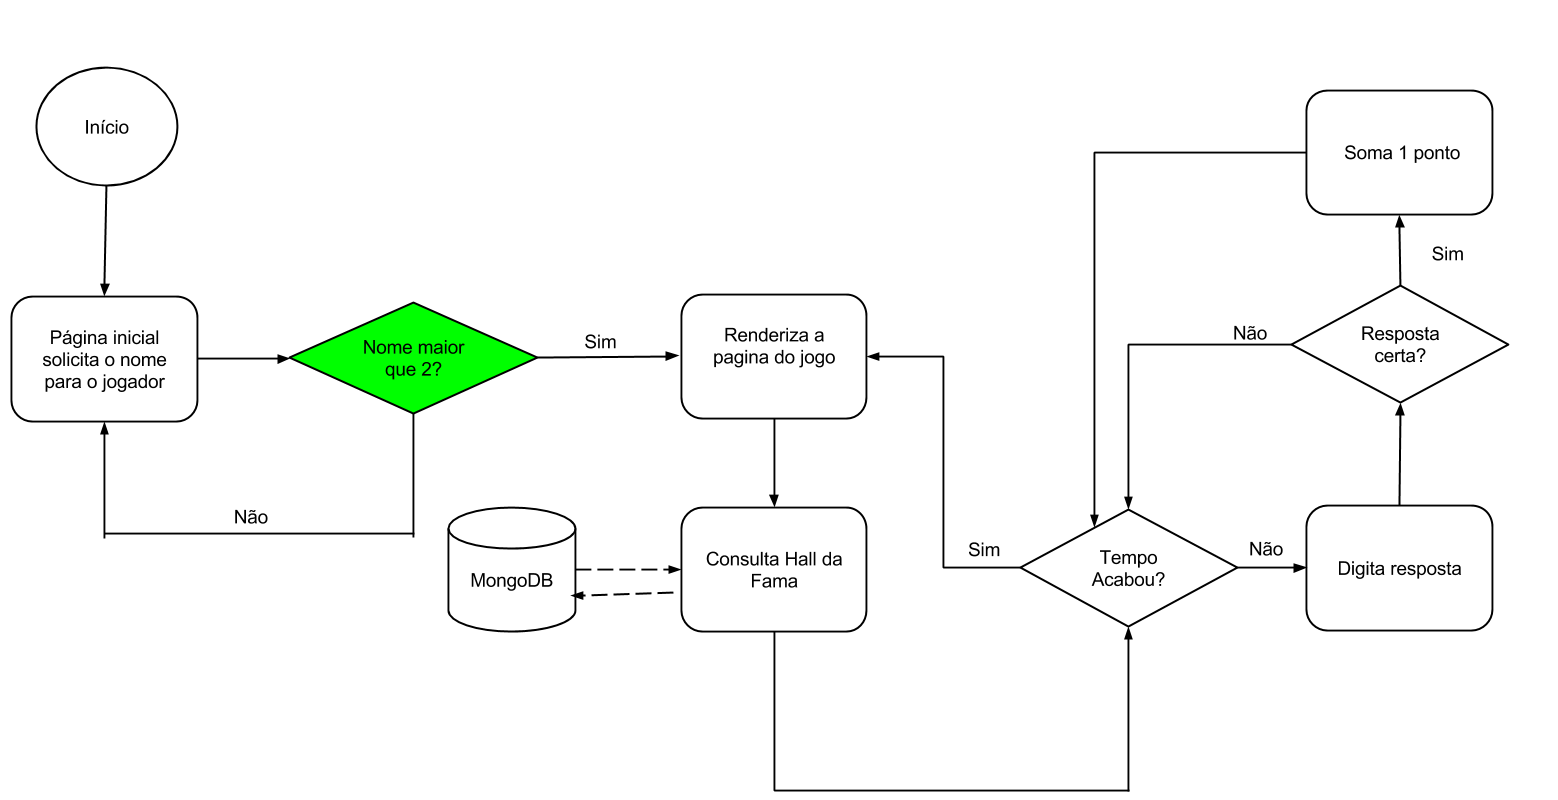
\includegraphics[scale=0.2]{../images/func_mr_s3.png}
    \caption{Diagrama do funcionamento da aplicação}
    \label{fig: func_mr3}
    \end{figure}
\end{frame}
\begin{frame}{Math Race - Fluxo de execução}
    \begin{figure}[htb]
    \centering
    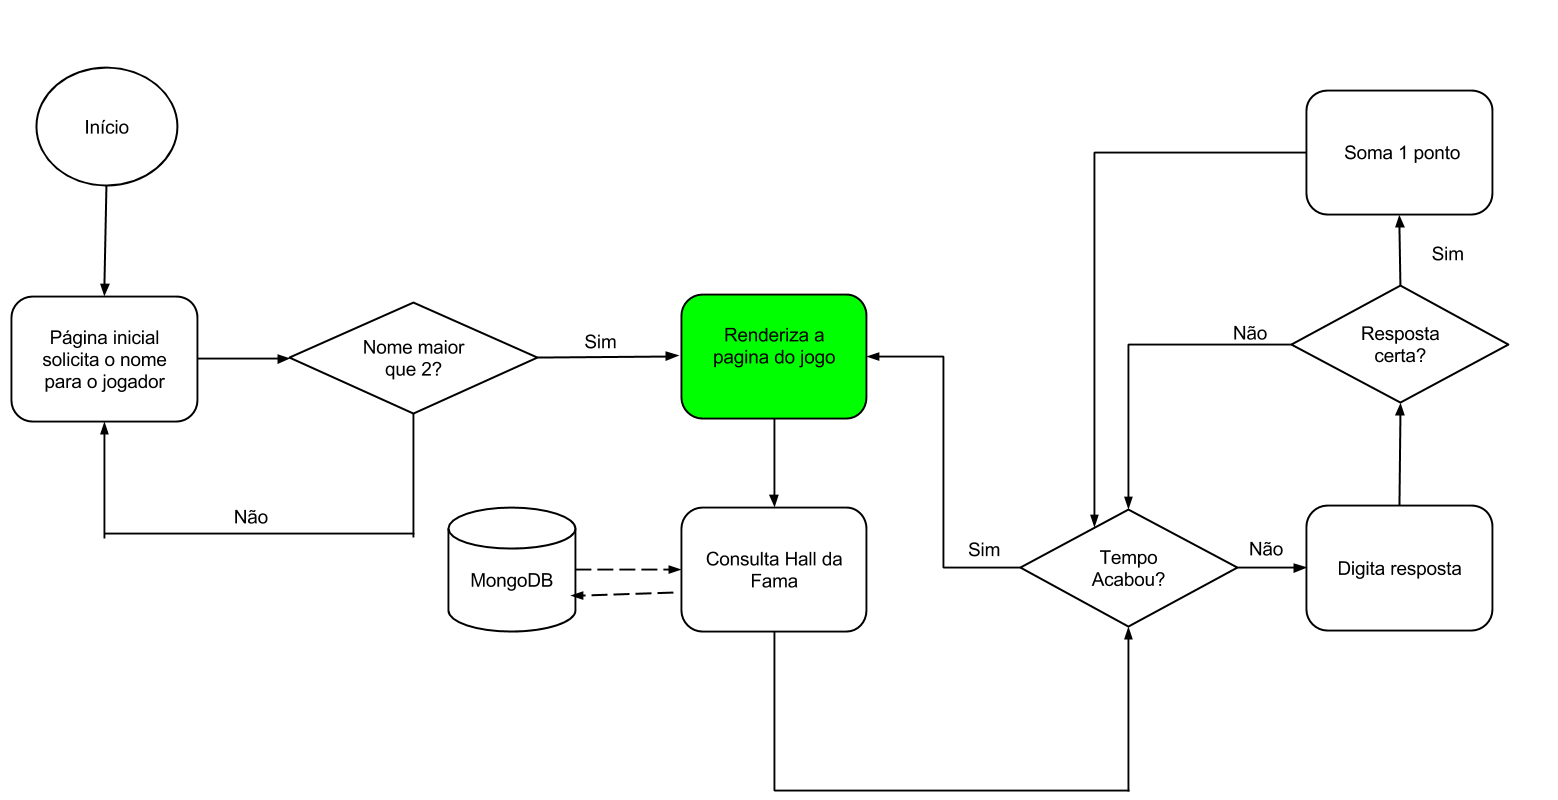
\includegraphics[scale=0.2]{../images/func_mr_s4.png}
    \caption{Diagrama do funcionamento da aplicação}
    \label{fig: func_mr4}
    \end{figure}
\end{frame}
\begin{frame}{Math Race - Fluxo de execução}
    \begin{figure}[htb]
    \centering
    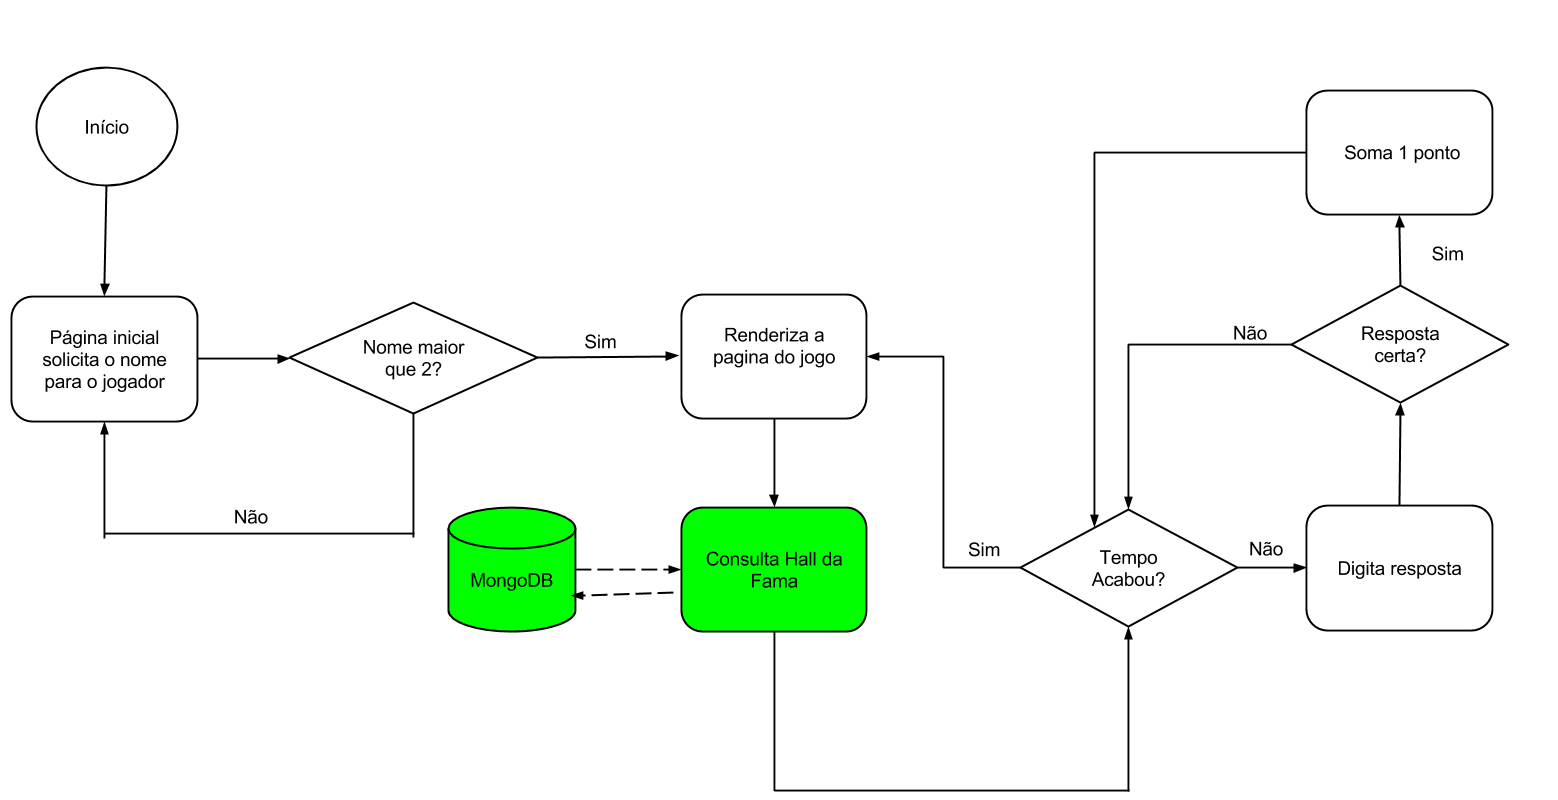
\includegraphics[scale=0.2]{../images/func_mr_s5.png}
    \caption{Diagrama do funcionamento da aplicação}
    \label{fig: func_mr5}
    \end{figure}
\end{frame}
\begin{frame}{Math Race - Fluxo de execução}
    \begin{figure}[htb]
    \centering
    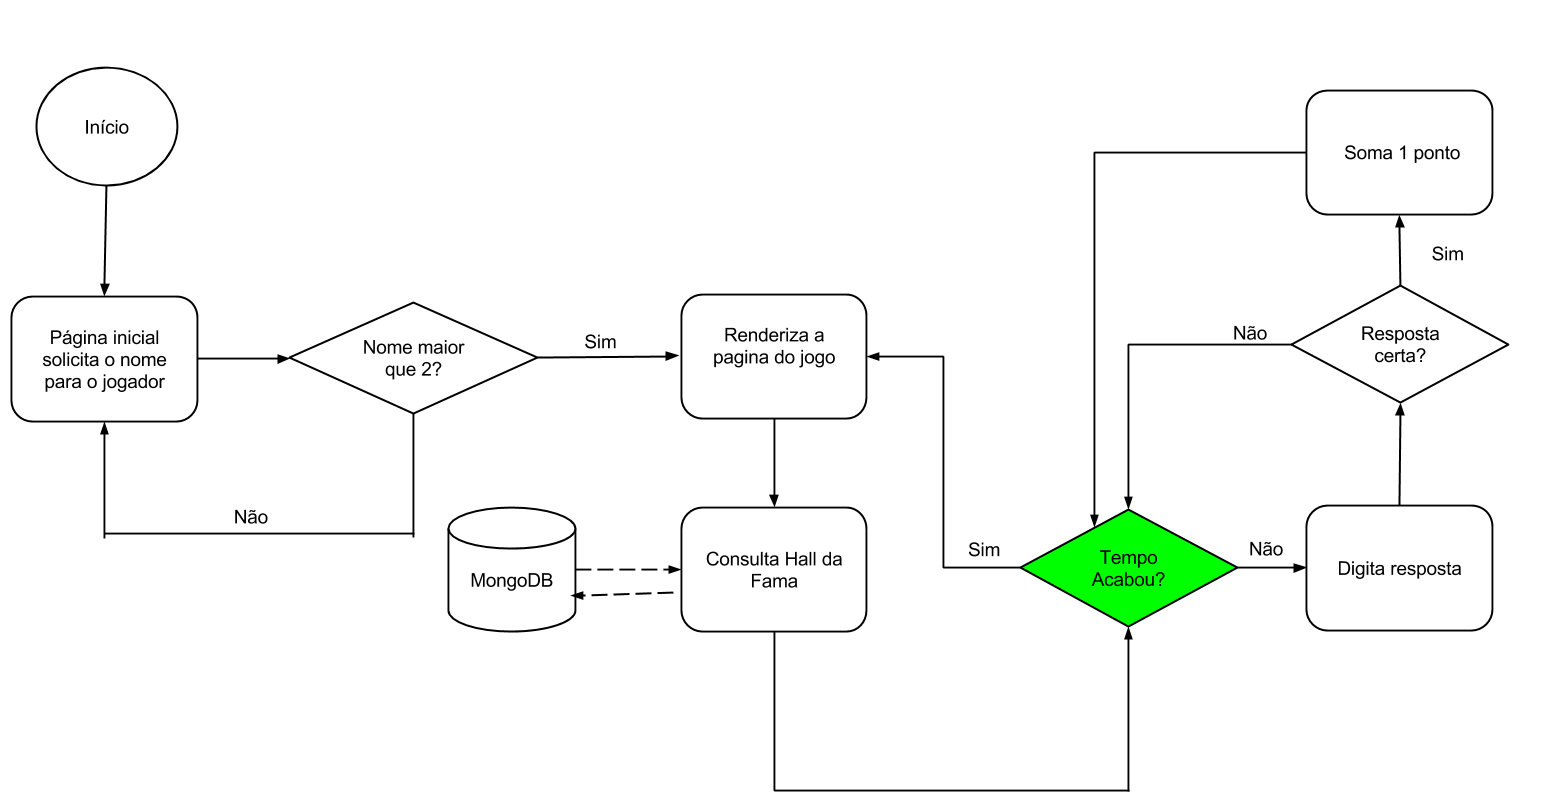
\includegraphics[scale=0.2]{../images/func_mr_s6.png}
    \caption{Diagrama do funcionamento da aplicação}
    \label{fig: func_mr6}
    \end{figure}
\end{frame}
\begin{frame}{Math Race - Fluxo de execução}
    \begin{figure}[htb]
    \centering
    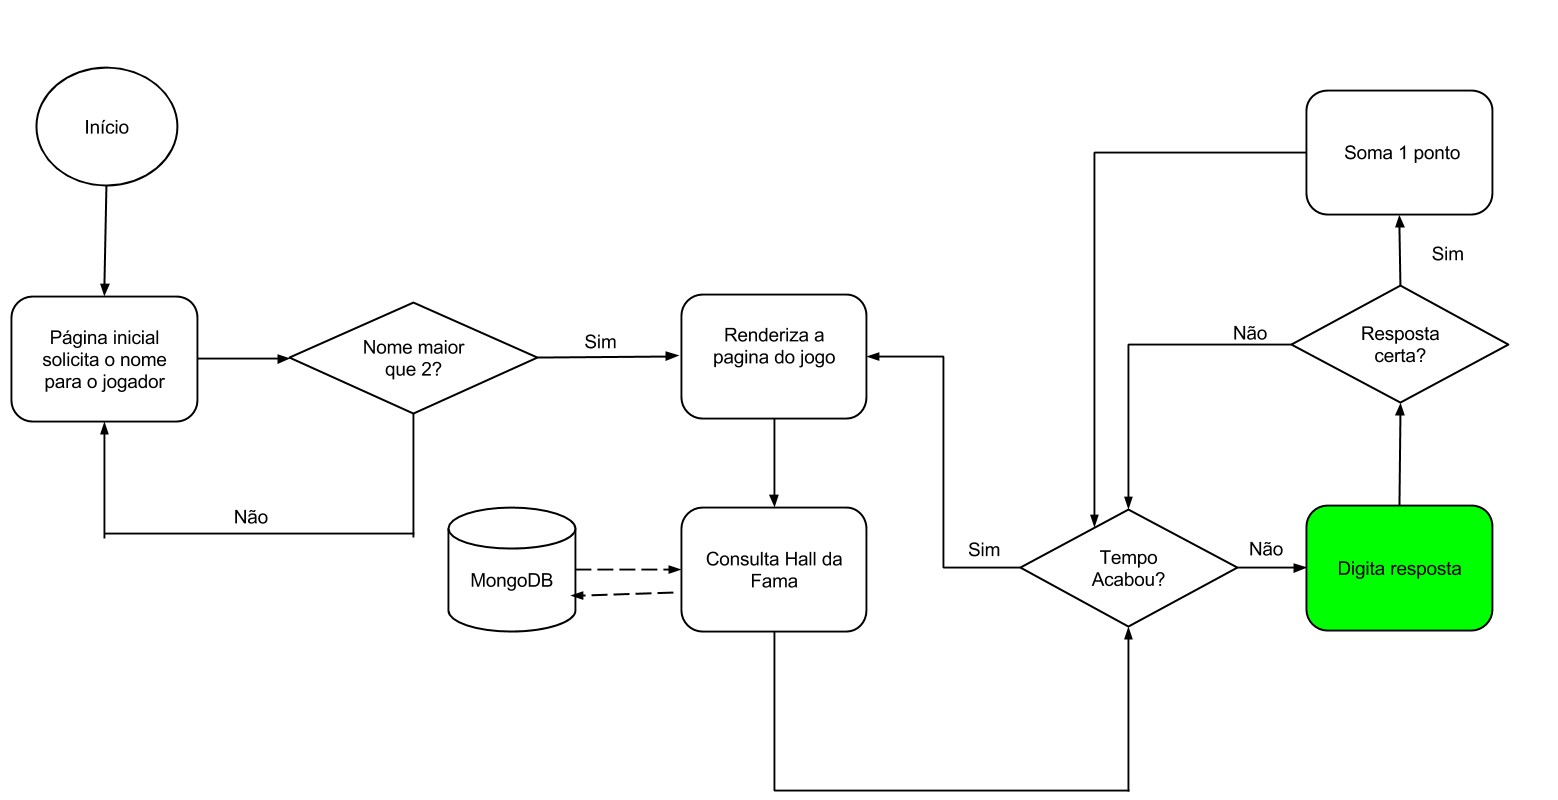
\includegraphics[scale=0.2]{../images/func_mr_s7.png}
    \caption{Diagrama do funcionamento da aplicação}
    \label{fig: func_mr7}
    \end{figure}
\end{frame}
\begin{frame}{Math Race - Fluxo de execução}
    \begin{figure}[htb]
    \centering
    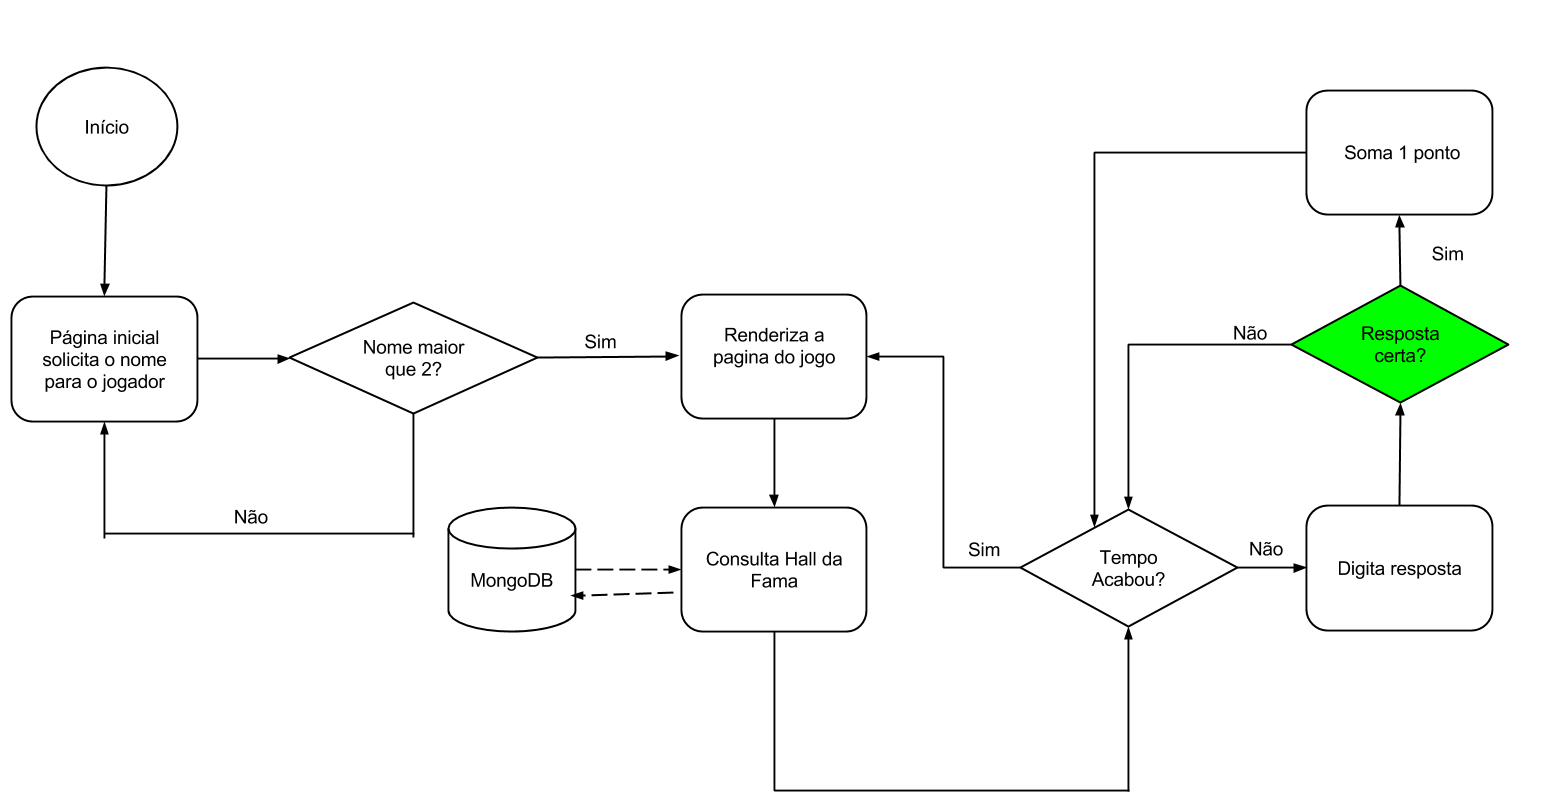
\includegraphics[scale=0.2]{../images/func_mr_s8.png}
    \caption{Diagrama do funcionamento da aplicação}
    \label{fig: func_mr8}
    \end{figure}
\end{frame}
\begin{frame}{Math Race - Fluxo de execução}
    \begin{figure}[htb]
    \centering
    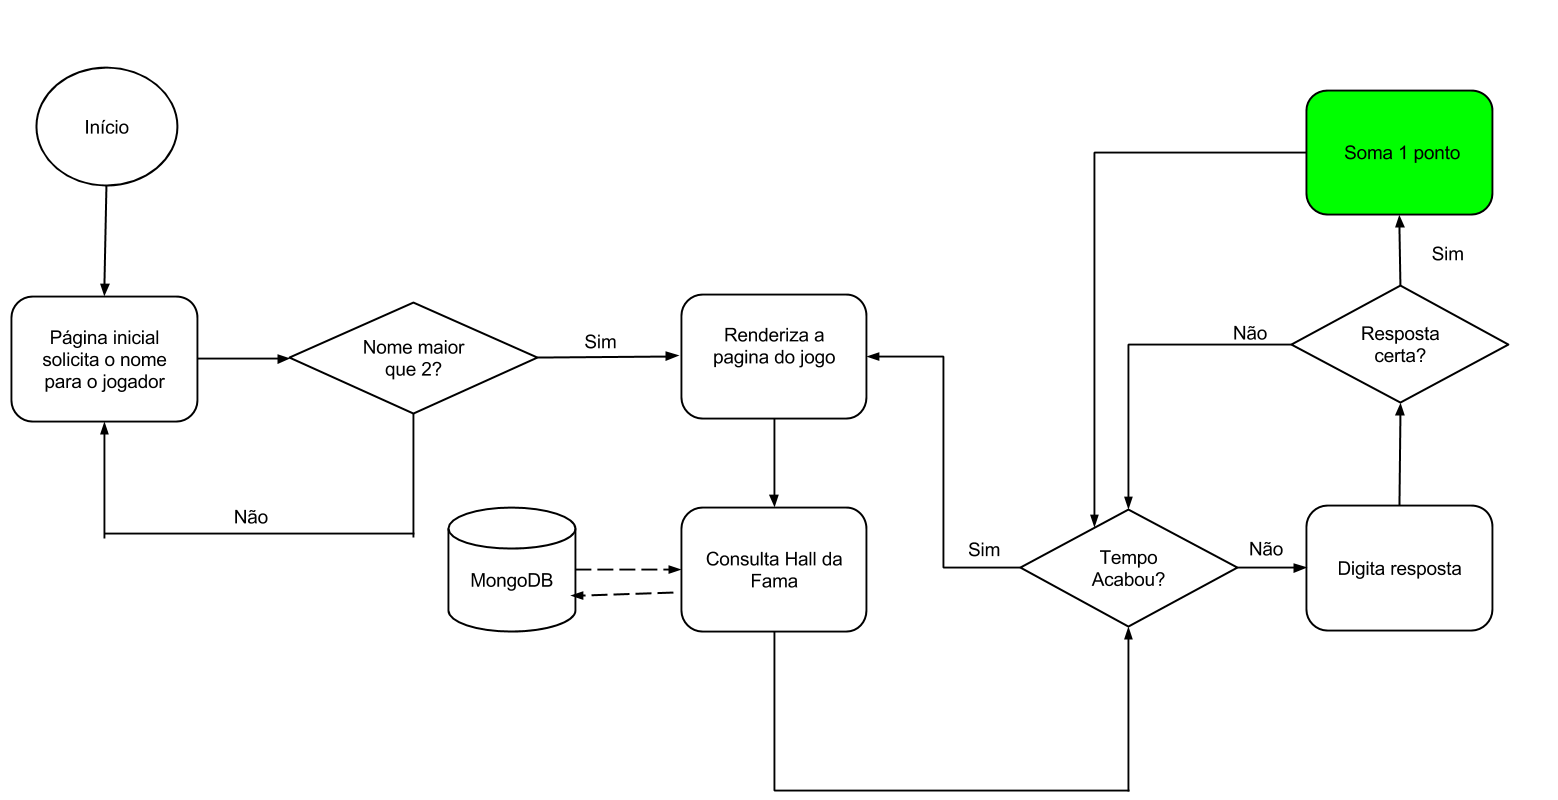
\includegraphics[scale=0.2]{../images/func_mr_s9.png}
    \caption{Diagrama do funcionamento da aplicação}
    \label{fig: func_mr9}
    \end{figure}
\end{frame}

%\begin{frame}{Testes de desempenho}
%Foram coletados \textit{fingerprints} de 67 locais distintos,
%  onde o incremento de um no eixo $x$ ou $y$ significa um metro do primeiro andar do DINF.
%\end{frame}

\begin{frame}{Math Race - Testes na Aplicação}
    \begin{figure}[htb]
    \centering
    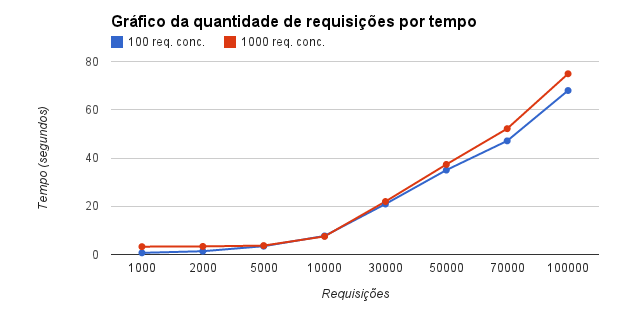
\includegraphics[scale=0.5]{../images/reqxtempo.png}
    \caption{Gráfico de requisições por tempo}
    \label{fig: grad_rq_tmp}
    \end{figure}
% Foram realizados 35 testes, onde:
%  \begin{itemize}
%      \item 22,8\% das estimativas possuem precisão de 1 metro ou menos.
%      \item 77,1\% das estimativas possuem precisão de 3 metros ou menos.
%      \item 91,4 \% das estimativas possuem precisão de 5 metros ou menos.
%     \end{itemize}
\end{frame}

\begin{frame}{Análise de testes de desempenho do Node.js e do MongoDB
com outros ambientes}
\begin{table}[htb]
\centering
\begin{tabular}{|c|c|c|}
\cline{1-3}
%\rowcolor[HTML]{CFCFCF}
Servidor & Linguagem de Programação & Banco de Dados \\ \cline{1-3}
Node.JS  & Javascript               & MongoDB        \\ \cline{1-3}
Node.Js  & Javascript               & PostgresSQL    \\ \cline{1-3}
Netty    & Java                     & MongoDB        \\ \cline{1-3}
Netty    & Java                     & PostgresSQL    \\ \cline{1-3}
Apache   & PHP                      & MongoDB        \\ \cline{1-3}
Apache   & PHP                      & PostgresSQL    \\ \cline{1-3}
\end{tabular}
\caption{Ambientes dos testes}
\label{fig: ap_amb_testes}
\end{table}
\end{frame}

\begin{frame}{Consumo de Memória RAM}
\begin{figure}[hbt]
  \centering
  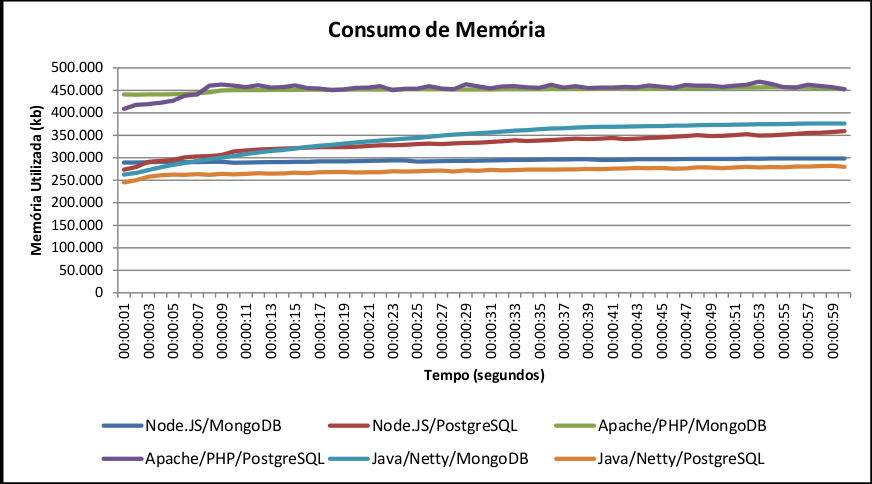
\includegraphics[scale=0.35]{../images/graf_memoria.png}
  \caption{ Consumo de memória RAM durante a execução dos teste.}
  \label{fig: consumo_ram}
  \end{figure}
\end{frame}

\begin{frame}{Utilização de CPU}
\begin{figure}[hbt]
  \centering
  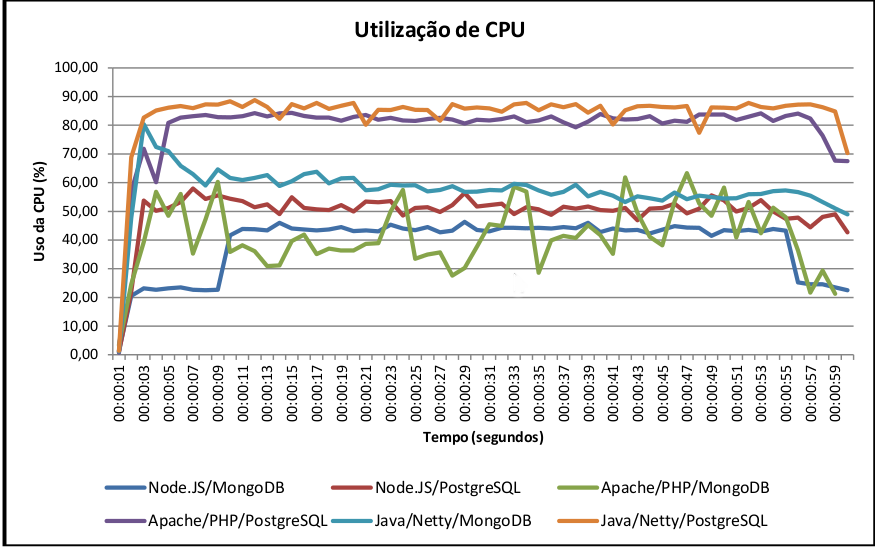
\includegraphics[scale=0.33]{../images/graf_cpu.png}
  \caption{Utilização de CPU}
  \label{fig: utilizacao_cpu}
  \end{figure}
\end{frame}

\begin{frame}{Quantidade de requisições por tempo}
\begin{figure}[hbt]
  \centering
  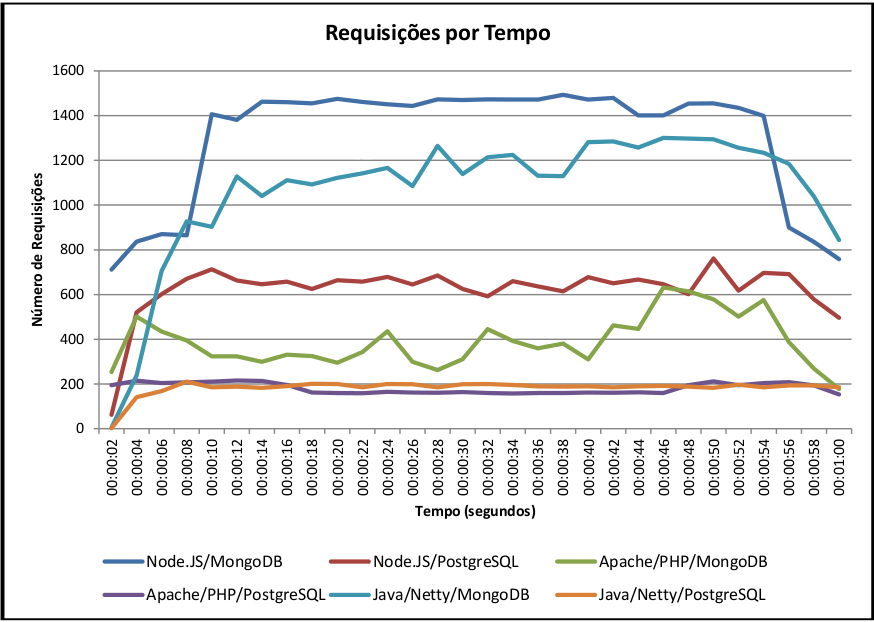
\includegraphics[scale=0.30]{../images/graf_req_tempo.png}
  \caption{Quantidade de requisições por tempo}
  \label{fig: req_tempo}
  \end{figure}
\end{frame}

\section{Conclusão}
\begin{frame}{Conclusão}

 O MEAN \textit{Stack} é de fato uma ótima opção para o desenvolvimento de aplicações web escaláveis, principalmente através do o Node.js e o MongoDB. 
 
 O Angular.js e o Express.js atuam como facilitadores no processo de desenvolvimento, sem estes componentes, dependendo da complexidade da aplicação, o tempo gasto no desenvolvimento da aplicação do lado do cliente pode aumentar drasticamente, e a utilização do Node.js pode ser consideravelmente mais trabalhosa. 
%\begin{itemize}
% \item Precisão satisfatória, considerando um raio de 2 até 5 metros da posição real do aparelho.
% \item A oscilação do RSS e a semelhança dos \textit{fingerprints} em um raio de até 5 metros do aparelho
%  dificultaram uma precisão mais aguda.
%  \item O ambiente deve ser lavado em consideração, já que o ambiente escolhido é bastante favorável a abordagem escolhida, dado
%      o grande número de APs presentes.
% \item Essa técnica pode ser bastante proveitosa na localização de robôs móveis, pois há 
%      a possibilidade de adicionar mais características para distinguir os \textit{fingerprints} com 
%      dados coletados por outros sensores do robô(câmera, laser, sonar).
%\end{itemize}
\end{frame}

\end{document}
